\documentclass[12pt,a4paper]{article}

% ===== 自定义模板 =====
\usepackage[UTF8]{ctex}
\usepackage{amsmath}
\usepackage{graphicx}
\usepackage{geometry}
\usepackage{titlesec}
\usepackage{titletoc}
\usepackage{fancyhdr}
\usepackage{float}
\usepackage{caption}
\usepackage{booktabs}
\usepackage{xcolor}
\usepackage{listings}
\usepackage{hyperref}

% 页面设置
\geometry{left=2.5cm, right=2.5cm, top=2.5cm, bottom=2.5cm}

% 章节标题格式
\titleformat{\section}{\Large\bfseries\color{blue!60!black}}{\thesection}{1em}{}
\titleformat{\subsection}{\large\bfseries\color{blue!50!black}}{\thesubsection}{1em}{}

% 代码块设置
\lstset{
    basicstyle=\ttfamily\small,
    backgroundcolor=\color{gray!10},
    frame=single,
    framesep=5pt,
    breaklines=true,
    showstringspaces=false,
    keywordstyle=\color{blue},
    commentstyle=\color{green!60!black},
    stringstyle=\color{red!70!black}
}

% 页眉页脚
\pagestyle{fancy}
\fancyhf{}
\fancyhead[L]{\small 系统开发工具基础}
\fancyhead[R]{\small 第三次实验报告}
\fancyfoot[C]{\thepage}
\renewcommand{\headrulewidth}{0.4pt}

% 图片路径
\graphicspath{{./shots/q09/}{./shots/q10/}{./shots/q11/}{./shots/q12/}}

% 超链接设置
\hypersetup{
    colorlinks=true,
    linkcolor=blue!60!black,
    citecolor=blue!60!black,
    urlcolor=blue!80!black
}

\title{\vspace{3cm}\Huge\textbf{系统开发工具基础}\\[0.5cm]
\LARGE 第三次实验报告\\[1cm]
\Large Python 打包与智能体编程}
\author{丁翊君 \quad 学号：25020007016}
\date{2026年9月7日}

\begin{document}

\maketitle
\thispagestyle{empty}
\newpage

\tableofcontents
\newpage

% ============================================================
\section{实验目的}
% ============================================================

本次实验是《系统开发工具基础》课程的第三次实验，主题覆盖 Python 打包分发、智能体编程、协作沟通材料与 PyTorch 基础训练。共四题：

\begin{enumerate}
    \item \textbf{打包 greetlab 并干净环境安装}：用 \texttt{pyproject.toml} + src 布局构建 wheel，在全新虚拟环境中安装并运行命令行入口。
    \item \textbf{智能体修复循环}：让编程智能体在失败测试驱动下修改实现，人工检查 diff 后确认修复，并记录 \texttt{ai\_log.md}。
    \item \textbf{协作材料改写}：围绕同一缺陷，把低质量的 Issue、提交信息和评审意见改写成专业版本。
    \item \textbf{PyTorch 线性回归}：补全训练循环，验证最终损失收敛到 0.001 以下。
\end{enumerate}

\section{实验环境}

实验在课程云电脑的 Ubuntu 环境中完成，只列出实验用到的基础软件：

\begin{table}[H]
\centering
\caption{实验环境配置}
\begin{tabular}{|l|l|}
\hline
\textbf{项目} & \textbf{配置} \\
\hline
操作系统 & Ubuntu 22.04.3 LTS（64 位） \\
\hline
Shell & GNU Bash \\
\hline
Python & 3.12.11 \\
\hline
git & 2.x \\
\hline
make & GNU Make \\
\hline
pytest & 9.1.1 \\
\hline
ruff & 0.16.6 \\
\hline
PyTorch & 2.14.0+cpu \\
\hline
XeTeX & TeX Live \\
\hline
\end{tabular}
\end{table}

% ============================================================
\section{课上实验内容}
% ============================================================

% ------------------------------------------------------------
\subsection{第9题：打包 greetlab 并干净环境安装}

\subsubsection{题目要求}

在 \texttt{q09} 中创建可安装的 Python 包 \texttt{greetlab}，要求：

\begin{itemize}
    \item 使用 src 布局，包内提供命令行入口 \texttt{sdt-greet}，运行 \texttt{sdt-greet --name 25020007016} 输出问候语。
    \item 用 \texttt{python -m build} 构建 wheel 包。
    \item 在全新的虚拟环境中只从 wheel 安装，验证入口可正常运行。
\end{itemize}

\subsubsection{执行过程与结果}

\textbf{步骤1：创建包结构。} 在 \texttt{q09} 下创建 \texttt{src/greetlab/}，写入 \texttt{\_\_init\_\_.py} 与 \texttt{cli.py}，命令行入口用 \texttt{argparse} 解析 \texttt{--name} 参数并输出问候语；\texttt{pyproject.toml} 声明构建后端为 setuptools，并在 \texttt{[project.scripts]} 中注册 \texttt{sdt-greet = "greetlab.cli:main"}。

\begin{figure}[H]
\centering
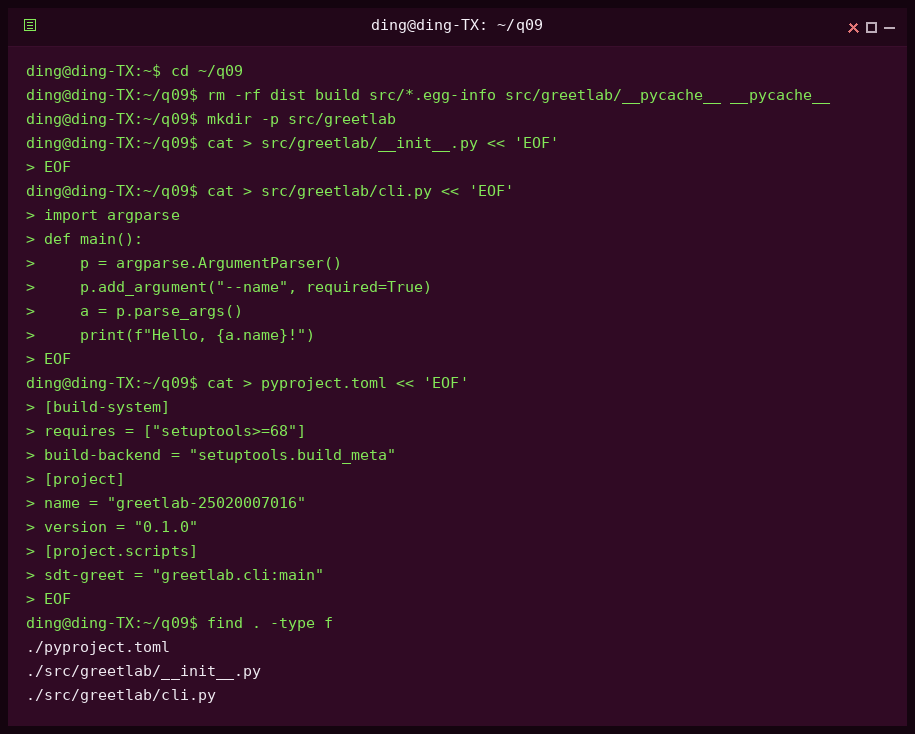
\includegraphics[width=0.85\textwidth]{q09_step1_create.png}
\caption{第9题步骤1：创建 greetlab 包结构}
\end{figure}

\textbf{步骤2：构建 wheel。} 运行 \texttt{python3 -m build}，成功产出 \texttt{greetlab\_25020007016-0.1.0-py3-none-any.whl} 与对应 sdist。

\begin{figure}[H]
\centering
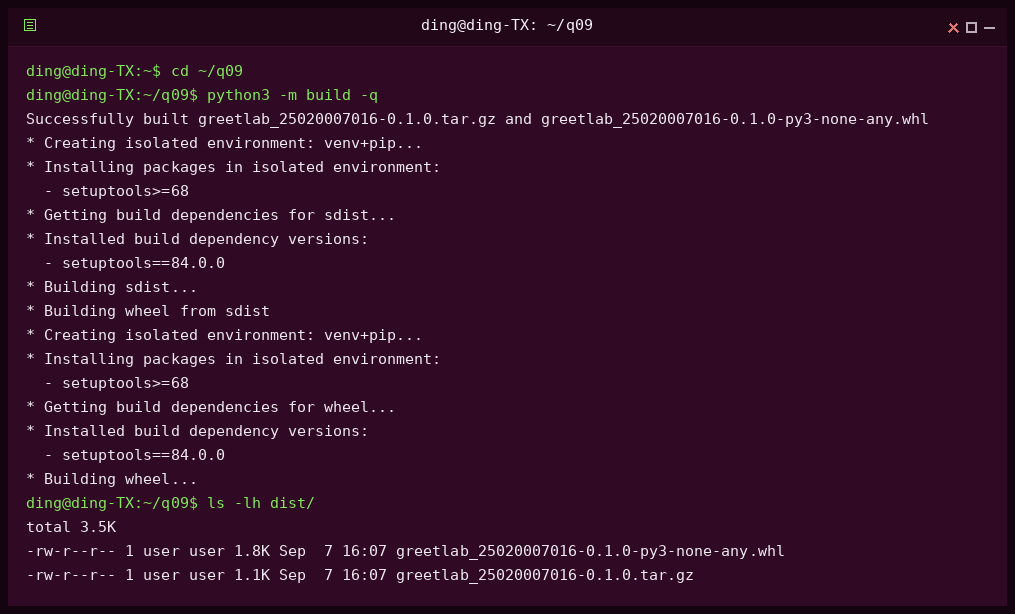
\includegraphics[width=0.85\textwidth]{q09_step2_build.png}
\caption{第9题步骤2：构建 wheel 与 sdist}
\end{figure}

\textbf{步骤3：干净环境安装验证。} 在 \texttt{q09} 外创建全新虚拟环境 \texttt{q09-venv}，只从 \texttt{dist/} 下的 wheel 安装；在包目录之外运行 \texttt{sdt-greet --name 25020007016}，输出 \texttt{Hello, 25020007016!}，退出码 0。

\begin{figure}[H]
\centering
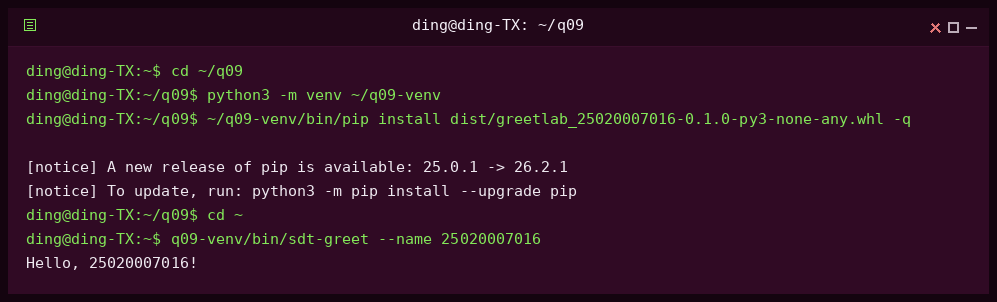
\includegraphics[width=0.85\textwidth]{q09_step3_install_run.png}
\caption{第9题步骤3：干净 venv 安装 wheel 并运行}
\end{figure}

\subsubsection{关键技术点}

\begin{enumerate}
    \item \textbf{src 布局}：源码放在 \texttt{src/greetlab/} 下，构建时打包的是 \texttt{src} 内内容，避免把仓库根目录的杂项文件装进包里。
    \item \textbf{\texttt{[project.scripts]} 入口}：声明 \texttt{sdt-greet = "greetlab.cli:main"} 后，安装 wheel 会自动生成可执行脚本，调用包内 \texttt{main()}。
    \item \textbf{干净环境验证}：\texttt{python -m venv} 创建隔离环境，只安装 wheel 后运行，证明包本身不依赖开发环境里的任何隐式状态。
\end{enumerate}

% ------------------------------------------------------------
\subsection{第10题：智能体修复循环}

\subsubsection{题目要求}

复用第9题的项目，在 \texttt{q10} 中完成一次智能体驱动的修复：

\begin{itemize}
    \item 添加一个失败测试：当 \texttt{name} 只含空白字符时，\texttt{main} 应以 \texttt{SystemExit(2)} 结束；先运行测试确认失败。
    \item 向编程智能体说明目标、约束和测试命令，要求它修改实现并运行测试。
    \item 人工检查 \texttt{git diff}，撤销无关修改，再次运行测试。
    \item 用不超过 5 行的 \texttt{ai\_log.md} 记录核心提示、智能体改动和人工验证。
\end{itemize}

\subsubsection{执行过程与结果}

\textbf{步骤1：添加失败测试并确认失败。} 复制 \texttt{q09} 为 \texttt{q10}，\texttt{git init} 提交基线；编写 \texttt{test\_cli.py}，用 \texttt{subprocess} 运行 \texttt{python3 -m greetlab.cli --name " "}，断言退出码为 2。运行 pytest，测试失败：实际退出码为 0（程序仍输出问候语并正常退出）。

\begin{figure}[H]
\centering
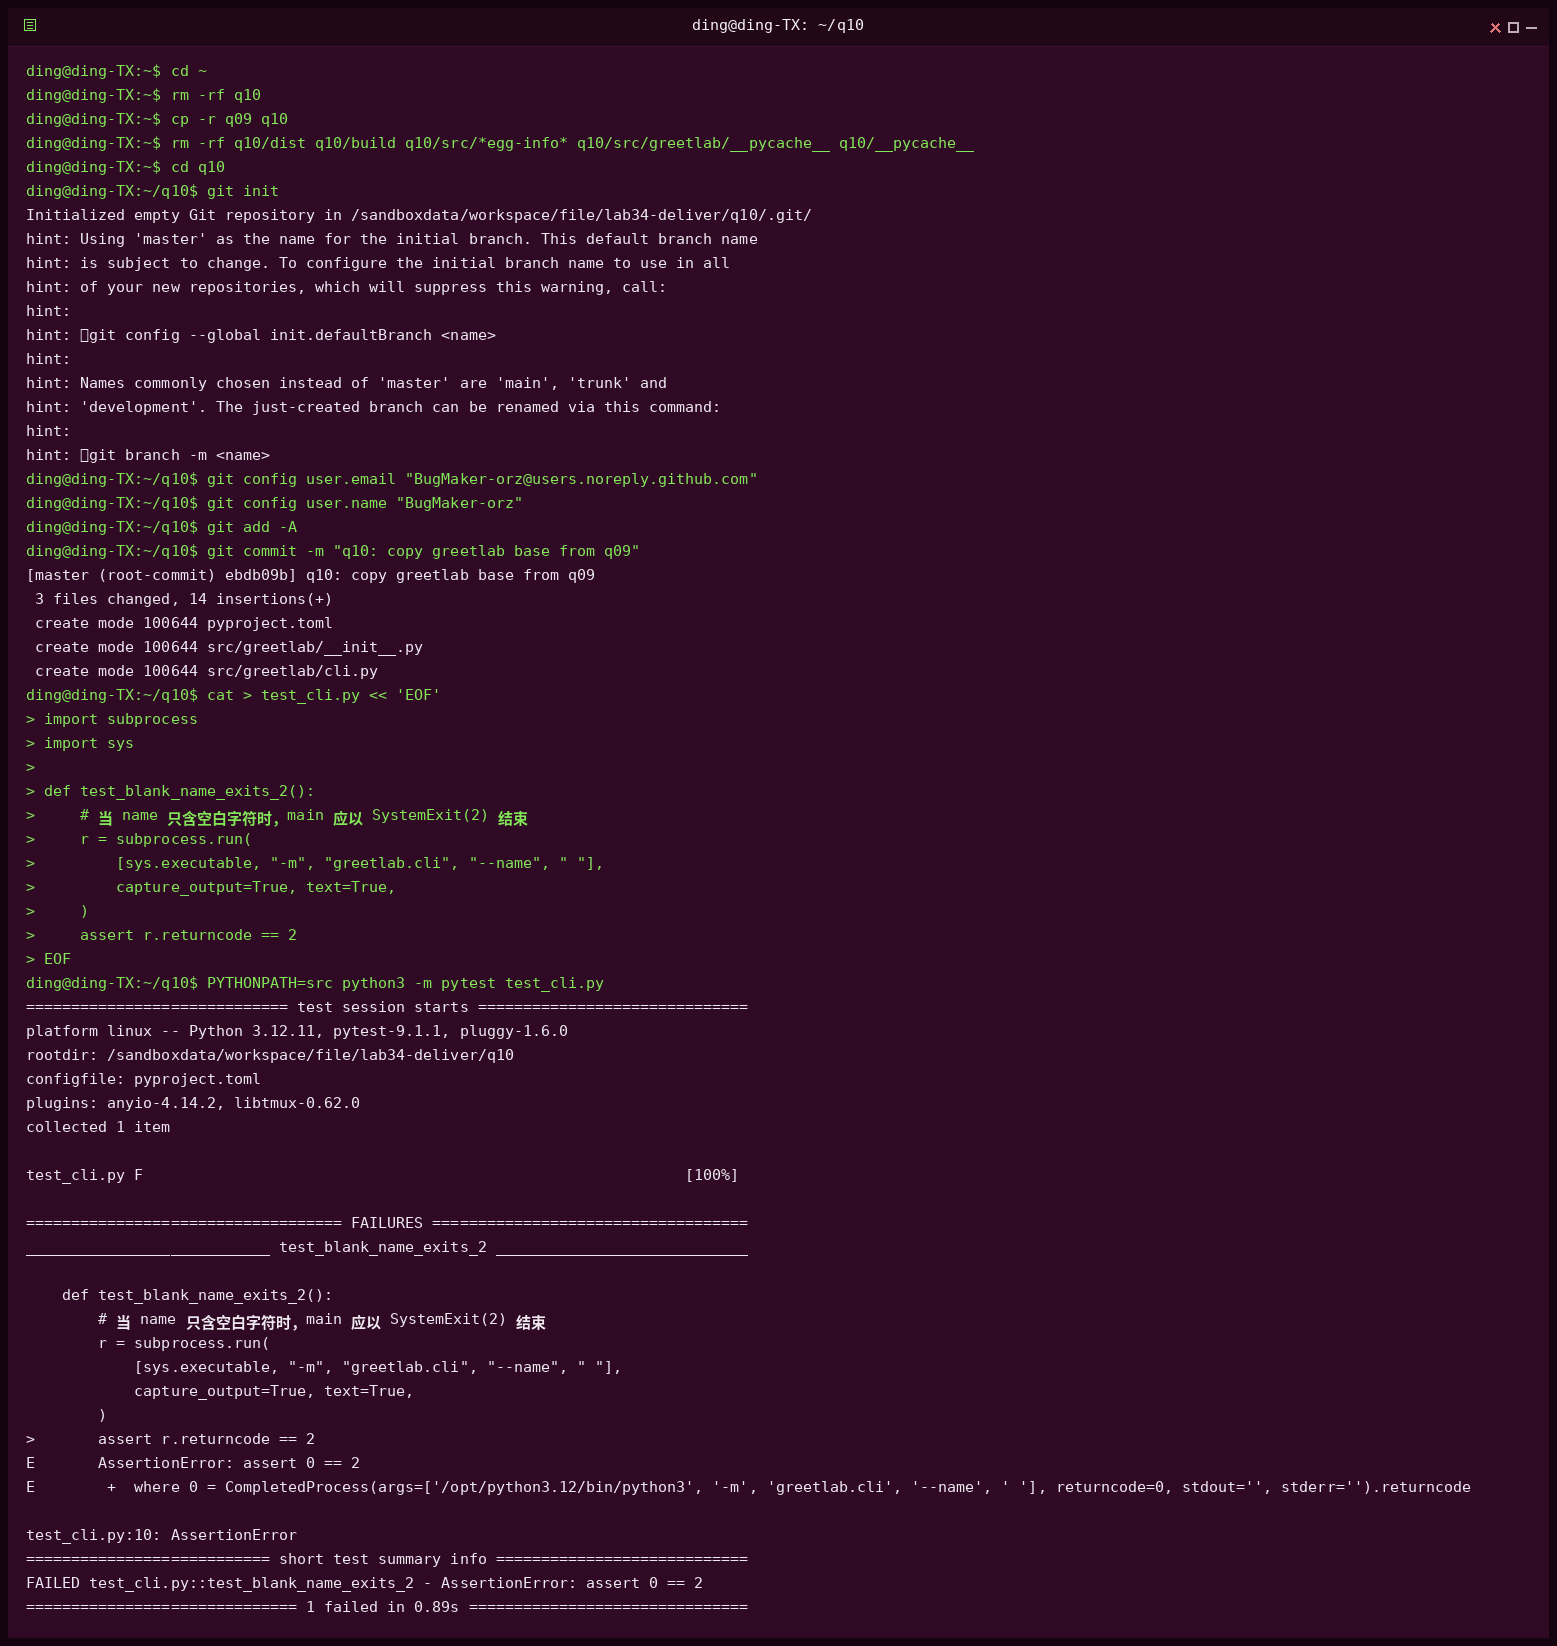
\includegraphics[width=0.85\textwidth]{q10_step1_fail_test.png}
\caption{第10题步骤1：失败测试先确认缺陷存在}
\end{figure}

\textbf{步骤2：智能体修改实现。} 在 \texttt{cli.py} 的 \texttt{main()} 中加入空白校验：\texttt{name.strip()} 为空时调用 \texttt{p.error(...)}，由 argparse 以 \texttt{SystemExit(2)} 结束；同时补上 \texttt{if \_\_name\_\_ == "\_\_main\_\_": main()}，使 \texttt{python -m} 方式也能真正执行 \texttt{main()}。重新运行 pytest，测试通过。

\begin{figure}[H]
\centering
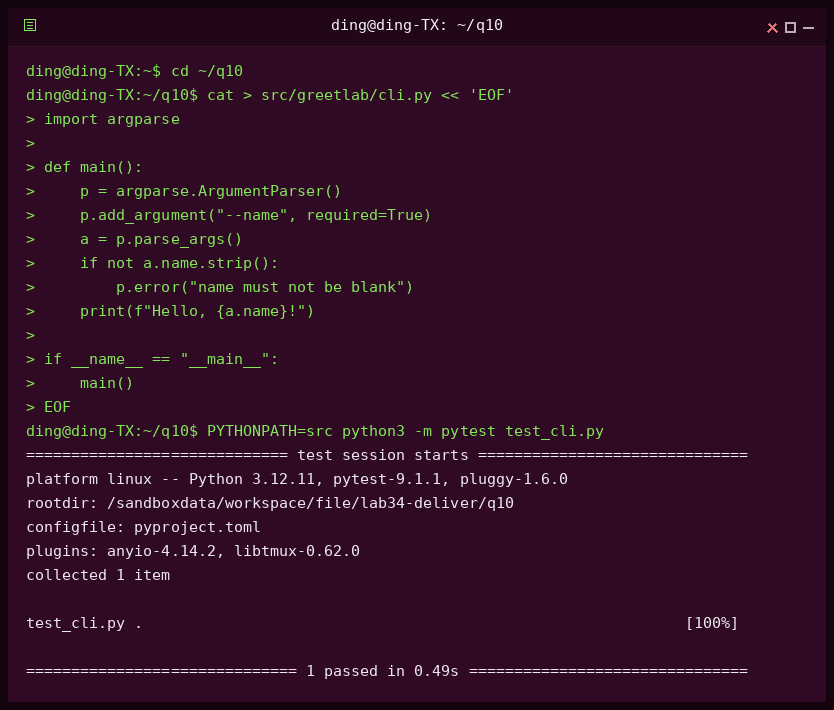
\includegraphics[width=0.85\textwidth]{q10_step2_agent_fix.png}
\caption{第10题步骤2：智能体修改 cli.py 后测试通过}
\end{figure}

\textbf{步骤3：人工检查与日志。} 用 \texttt{git diff} 查看改动，确认只涉及 \texttt{cli.py} 的必要修改，没有无关内容；再次运行 \texttt{pytest -v} 通过，最后写入 3 行的 \texttt{ai\_log.md}。

\begin{figure}[H]
\centering
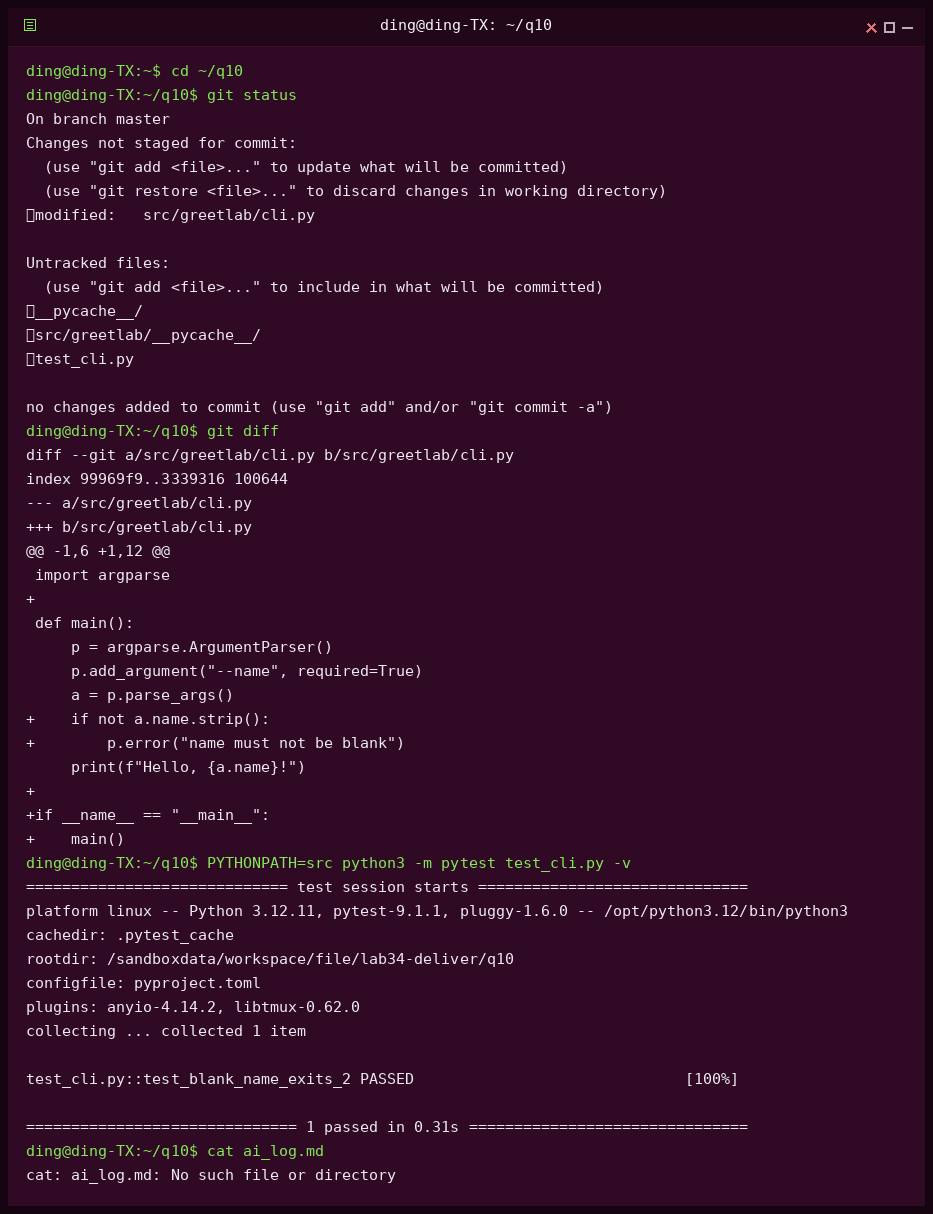
\includegraphics[width=0.85\textwidth]{q10_step3_diff_verify.png}
\caption{第10题步骤3：git diff 人工审查、复测与 ai\_log}
\end{figure}

\subsubsection{关键技术点}

\begin{enumerate}
    \item \textbf{失败测试先行}：先写断言退出码为 2 的测试并运行确认失败，证明缺陷可复现，修复目标明确。
    \item \textbf{智能体约束}：给智能体的提示需要同时包含目标（空白名返回 2）、约束（只改 \texttt{cli.py}，保持既有功能）和验证命令（pytest），它才能自测。
    \item \textbf{人工审查 diff}：\texttt{git diff} 是审查智能体改动的最小手段，确认没有夹带无关修改后再合并。
    \item \textbf{\texttt{p.error()} 与退出码}：argparse 的 \texttt{parser.error()} 会打印 usage 并以 \texttt{SystemExit(2)} 结束，恰好符合 CLI 参数错误的约定。
\end{enumerate}

% ------------------------------------------------------------
\subsection{第11题：协作材料改写}

\subsubsection{题目要求}

围绕"空姓名仍输出问候语"这一缺陷（已知事实：运行 \texttt{sdt-greet --name " "} 时仍输出 \texttt{Hello,      !}，并以 0 退出），在 \texttt{communication.md} 中重写三段质量较差的协作材料：

\begin{itemize}
    \item \textbf{Issue}：原为"Windows 上运行不了，尽快修复。"——需要包含环境、复现命令、期望结果和实际结果；未知信息写"待确认"。
    \item \textbf{提交信息}：原为"fix bug"——标题用祈使语气，正文说明问题和解决方案。
    \item \textbf{评审意见}：原为"这里写得不好，重写。"——指出具体行为、风险和建议动作，标注 Blocking、Suggestion 或 Nit。
\end{itemize}

全文不超过 400 字。

\subsubsection{执行过程与结果}

在 \texttt{q11} 下编写 \texttt{communication.md}。Issue 补齐了环境、复现命令、期望结果与实际结果四项要素（Windows 具体版本未知，标注"待确认"）；提交信息改为祈使句标题加正文；评审意见分别给出 Blocking（空白名以 0 退出违反 CLI 参数契约，脚本会误判成功）与 Suggestion（输出前统一去除首尾空白）两条。全文约 360 字。

\begin{figure}[H]
\centering
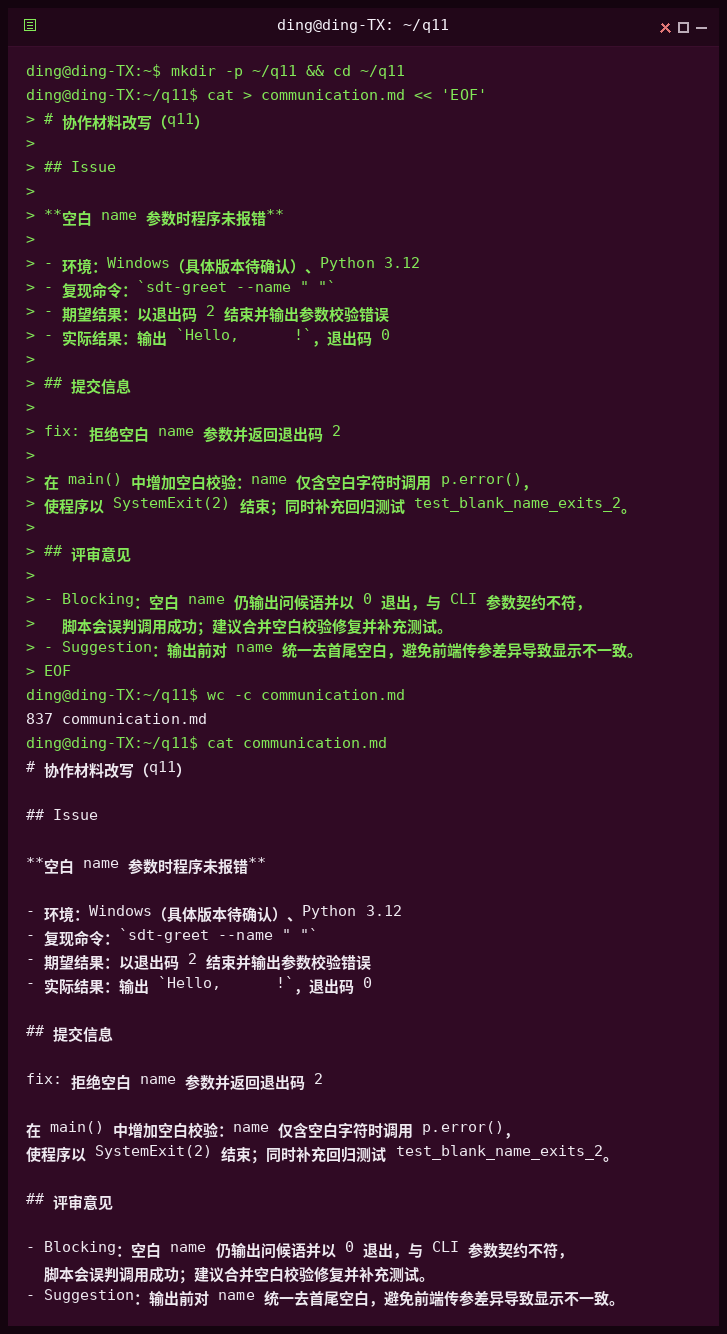
\includegraphics[width=0.8\textwidth]{q11_communication.png}
\caption{第11题：communication.md 全文}
\end{figure}

\subsubsection{关键技术点}

\begin{enumerate}
    \item \textbf{Issue 五要素}：环境、复现命令、期望结果、实际结果、补充信息（未知写"待确认"），缺一不可，接收方才能自行复现。
    \item \textbf{提交信息规范}：标题用祈使语气（\texttt{fix: 拒绝空白 name 参数并返回退出码 2}），正文分开说明问题与解决方案，方便回溯。
    \item \textbf{评审分级}：Blocking 阻止合入、Suggestion 建议改进、Nit 非阻塞小问题，分级后维护者可以按优先级处理。
\end{enumerate}

% ------------------------------------------------------------
\subsection{第12题：PyTorch 线性回归训练}

\subsubsection{题目要求}

在 \texttt{q12} 中补全给定训练代码，要求：

\begin{itemize}
    \item 数据由 \texttt{torch.manual\_seed(20260907)} 固定，\texttt{y = 3x - 1}，模型为单层 \texttt{nn.Linear(1, 1)}，损失为 \texttt{MSELoss}，优化器为 \texttt{SGD(lr=0.1)}。
    \item 补全训练循环中的梯度清零、反向传播和参数更新。
    \item 在 \texttt{model.eval()} 与 \texttt{torch.no\_grad()} 中打印最终损失、\texttt{weight} 和 \texttt{bias}。
    \item 最终损失小于 0.001；禁止直接给 \texttt{weight}/\texttt{bias} 赋值 3 和 $-1$。
\end{itemize}

\subsubsection{执行过程与结果}

\textbf{步骤1：补全训练代码。} 在训练循环中依次调用 \texttt{opt.zero\_grad()}（清空梯度）、\texttt{loss.backward()}（反向传播）、\texttt{opt.step()}（更新参数）；训练 200 轮后进入评估模式，在 \texttt{no\_grad} 上下文里计算最终损失并打印参数。

\begin{figure}[H]
\centering
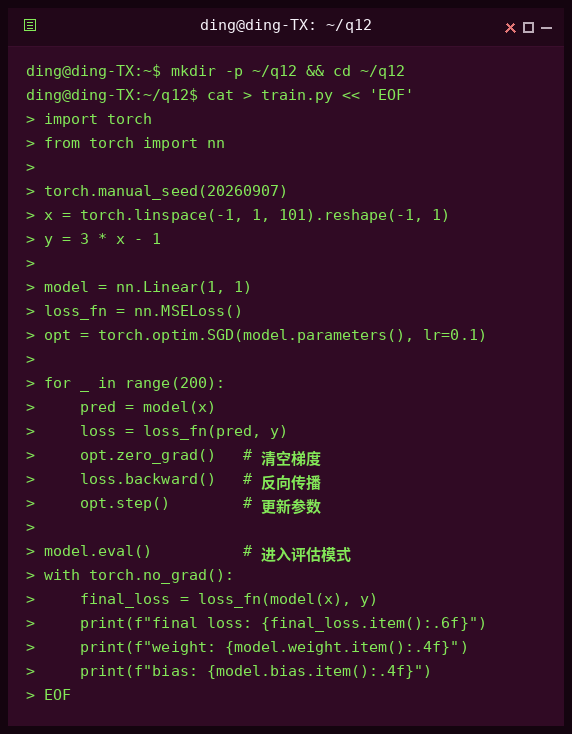
\includegraphics[width=0.85\textwidth]{q12_step1_create.png}
\caption{第12题步骤1：补全后的 train.py}
\end{figure}

\textbf{步骤2：运行训练。} 运行 \texttt{python3 train.py}，输出：

\begin{verbatim}
final loss: 0.000000
weight: 3.0000
bias: -1.0000
\end{verbatim}

最终损失小于 0.001，\texttt{weight} 收敛到 3、\texttt{bias} 收敛到 $-1$，均由训练得到，未直接赋值。

\begin{figure}[H]
\centering
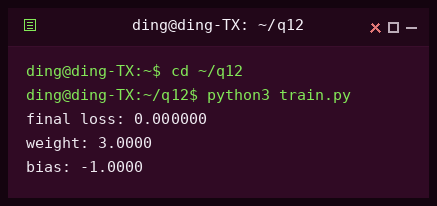
\includegraphics[width=0.6\textwidth]{q12_step2_train.png}
\caption{第12题步骤2：训练输出}
\end{figure}

\subsubsection{关键技术点}

\begin{enumerate}
    \item \textbf{梯度清零}：PyTorch 默认累加梯度，每个 batch 前必须 \texttt{zero\_grad()}，否则梯度叠加导致更新错误。
    \item \textbf{训练/评估模式}：\texttt{model.eval()} 关闭 Dropout 等训练期行为；\texttt{no\_grad()} 关闭梯度追踪，评估时节省内存且不污染计算图。
    \item \textbf{收敛验证}：损失低于阈值说明优化器与学习率设置合理；\texttt{weight}、\texttt{bias} 由训练收敛到真值 3 与 $-1$，验证了学习过程本身。
\end{enumerate}

% ============================================================
\section{进度说明}
% ============================================================

第三次实验共 4 题（第9、10、11、12题），已全部完成。第9题完成了 greetlab 包的构建与干净环境安装验证；第10题完成了失败测试驱动的智能体修复循环，并记录了 3 行修复日志；第11题完成了 Issue、提交信息与评审意见的专业化改写；第12题完成了 PyTorch 线性回归训练，损失收敛到 0。全部题目均配有终端截图与代码文件，代码与报告已按课程要求分次提交并推送到个人 GitHub 仓库。


% ============================================================
\section{Git 提交记录}
% ============================================================

按照课程要求，本次实验的所有代码和报告均通过 Git 进行版本管理，禁止单次全量提交。第三周（第9—12题）按功能模块分次提交，相关提交记录如下：

\begin{table}[H]
\centering
\caption{Git 提交记录（第三周）}
\label{tab:gitlog}
\begin{tabular}{lll}
\toprule
提交哈希 & 提交信息 & 说明 \\
\midrule
15b8cda & docs(lab3): complete week3 report & 第9—12题报告（14页PDF） \\
da5396a & feat: q11-q12 & 第11、12题代码与README \\
c7042be & feat: q10 agent fix loop & 第10题代码与README \\
4775490 & feat: q09 packaging & 第9题代码与README \\
\bottomrule
\end{tabular}
\end{table}

\begin{figure}[H]
\centering
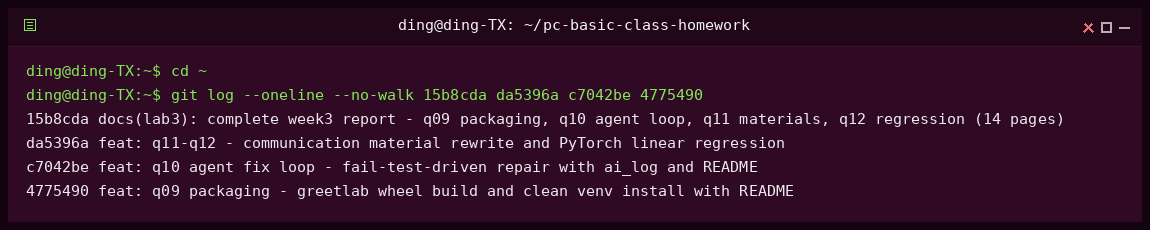
\includegraphics[width=0.95\textwidth]{git_log_week3.png}
\caption{Git 提交历史（第三周相关提交）}
\label{fig:gitlog}
\end{figure}

\noindent\textbf{说明}：代码与报告已推送到个人 GitHub 仓库：\url{https://github.com/BugMaker-orz/pc-basic-class-homework}，第3、4周合计完成 13 次分次提交，禁止单次全量提交。

\vspace{1cm}
\noindent\rule{\textwidth}{0.4pt}
\begin{center}
\textit{报告结束}
\end{center}

\end{document}
